\documentclass[11pt,oneside,openany]{book}
\usepackage{zlc_frontend_notes}

\begin{document}
\frontmatter
\zlctitlepage{PythonCamDemo / address\_switch 控制逻辑迁移说明}{原始控制代码解析与 Zou\_lab\_control 重构设计}{qCMOS、AOD/PXIE、重排、FPGA 时序、实验调度与可追溯性}{2026-05-31}
\tableofcontents
\cleardoublepage
\mainmatter


\chapter{阅读范围与结论}
\section{这份文档只讨论什么}
这份说明书只讨论两个原始控制代码来源：\filepath{PythonCamDemo} 和 \filepath{address_switch}。前者是中性原子实验中 qCMOS、AOD/PXIE、重排、校准和 notebook 试验流程的 Python 代码；后者是 FPGA/Vivado 工程中用 VIO 参数和 \pyapi{time_count} 累计条件产生 TTL、shutter 和 DA 输出的 Verilog 控制逻辑。Confocal GUI 的 device/logic/live\_plot 框架不是这里的原始控制逻辑，因此本文不会展开它的 GUI 架构。

\section{一句话总结}
原始代码的核心思想是正确的：用 qCMOS 外触发拍图，用阱中心和阈值判断 loading，用匈牙利匹配和路径规划决定重排，用 PXIE 的 ramp table 移动 AOD tweezer，用 FPGA 的硬时序输出 MOT、PGC、probe、microwave、pushout 和相机触发相关 TTL。问题不在实验物理流程，而在软件边界：硬件 IO、图像分析、路径规划、显示、保存和时序生成经常在同一个 notebook cell 或函数里直接串起来，状态靠当前目录、全局变量、\filepath{.npy} 文件和手写累计时间表达式隐式传递。

重构后的 \pyapi{Zou_lab_control.neutral_atom} 做的事，是把这些隐式状态拆成几个明确协议：
\begin{itemize}
  \item qCMOS 变成 \pyapi{HamamatsuQCMOSCamera} 和 \pyapi{QCMOSConfig}，采集生命周期按 \pyapi{validate -> prepare -> arm -> fire -> read -> stop} 执行。
  \item FPGA 时序变成 \pyapi{PulseSequence -> edge table -> VerilogBuild}，秒级物理时序和 tick 级硬件投影分开。
  \item AOD/PXIE 变成 \pyapi{FrequencyMap}、\pyapi{AODMove}、\pyapi{plan_move} 和 \pyapi{PXIEAOD}，site planner 与 DLL ramp 上传分开。
  \item 图像判别变成 \pyapi{TrapCalibration}、\pyapi{roi_counts}、\pyapi{detect_atoms}，旧的 \filepath{center.npy/threshold.npy/freq.npy} 变成显式可记录的校准对象。
  \item 实验调度变成 \pyapi{ShotExperiment}、\pyapi{ImageStackExperiment}、\pyapi{LoadingHistogramExperiment}、\pyapi{RabiExperiment} 和 \pyapi{RearrangementExperiment}，每个实验返回结果 dataclass，而不是直接把存图、画图和硬件句柄混在一起。
  \item notebook/live 显示变成 \pyapi{Zou_lab_control.frontend} 的 array 契约和 \pyapi{RunSession}，采集 worker 不碰 Matplotlib，UI timer 不读硬件。
\end{itemize}

\begin{notebox}[维护者读法]
读这份文档时不要把它当成 API 索引，而要看“状态在哪里拥有、什么时候跨层传递、失败时从哪里查”。中性原子控制最容易坏的地方不是某个函数少一行，而是 qCMOS armed 状态、FPGA 输出状态、PXIE ramp 状态、图像分析状态和 notebook figure 状态互相混在一起。
\end{notebox}

\chapter{原始 PythonCamDemo 总览}
\section{目录角色}
\filepath{PythonCamDemo} 里真正构成控制链的文件可以按下面理解：
\begin{description}
  \item[\filepath{qCMOS.py}] qCMOS 外触发采集主入口，包含实时显示进程、DCAM 初始化、ROI 配置、多帧 buffer、保存 TIFF、按 sub-frame 平均。
  \item[\filepath{qCMOS_ImageLive.py}] 与 \filepath{qCMOS.py} 非常接近，但加入 \pyapi{keep_camera_open} 的全局相机复用思路。
  \item[\filepath{dcam_live_capturing.py} 与 \filepath{Trigger.py}] DCAM SDK 示例和注释，说明 STABLE/READY、软件/外部触发、cap\_start、wait frame、buffer 读取这些底层状态。
  \item[\filepath{calculate.py}] site ROI 判别、target 列表、邻接图、带占用惩罚的路径搜索和 cascade pushing 版本的重排逻辑。
  \item[\filepath{compress_algorithm.py}] 更早的 5x5 grid 匈牙利匹配、折线路径插点、路径重排和路径拆分逻辑。
  \item[\filepath{pxie_control.py}] PXIE DLL 绑定、静态 SSB 参数、RA ramp 参数、两轴频率运动、丢弃原子和 move 执行。
  \item[\filepath{frequen_set.py}] 把 \filepath{freq.npy} 里的频率表按旧 notebook 约定翻转和整理成两轴频率列表。
  \item[\filepath{Auto_match.py} 与 \filepath{analyze.py}] 静态阱中心识别、阈值估计、Basler/SLM/AOD 校准相关流程。
  \item[\filepath{2D_rearrangement.ipynb}] 把以上函数串成真实实验流程的 notebook：打开相机和板卡、拍校准图、加载阈值和频率、测试 move、执行正式重排。
\end{description}

\section{原始流程的状态图}
\begin{figure}[htbp]
  \centering
  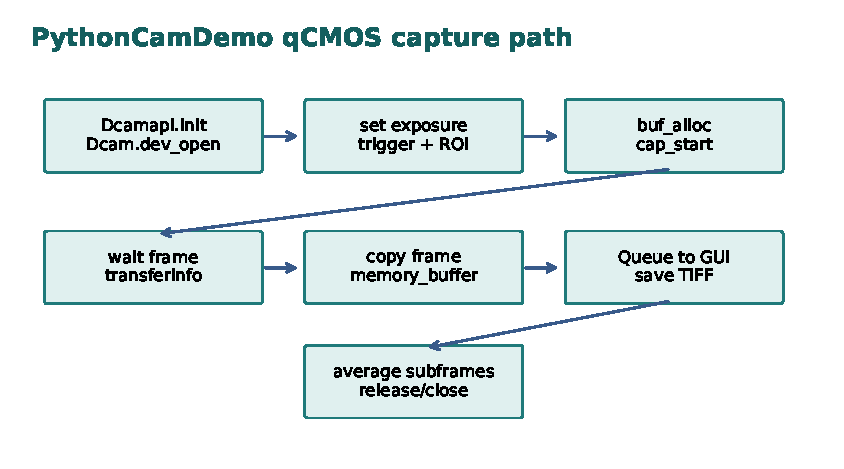
\includegraphics[width=0.96\textwidth]{assets/original_qcmos_flow.pdf}
  \caption{原始 qCMOS 采集函数把 DCAM 生命周期、GUI 进程、内存保存和平均图计算放在同一个函数内。}
\end{figure}

\begin{figure}[htbp]
  \centering
  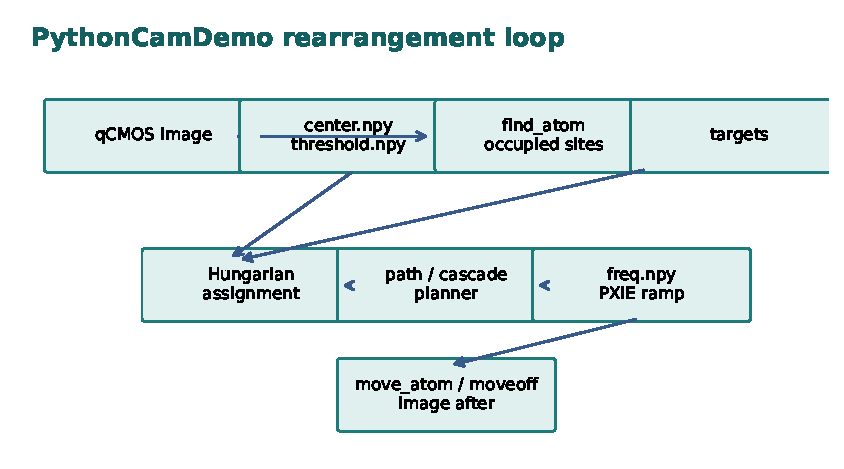
\includegraphics[width=0.96\textwidth]{assets/original_rearrange_flow.pdf}
  \caption{原始重排 notebook 的主线：拍图、阈值判别、规划路径、读取频率表、PXIE 执行、再次拍图验证。}
\end{figure}

\section{原始代码为什么能快速推进实验}
原始代码非常适合早期实验探索。它把每一步都写成 notebook 里可以马上运行的函数或 cell：相机拍照失败可以直接 print，AOD 频率可以手动改，某个 site 的移动可以单独测试，阈值和中心点可以保存成 \filepath{.npy} 立即复用。对于还在调硬件连线、寻找 trap center、试 PXIE ramp 参数的阶段，这种脚本式结构很高效。

它的另一个优点是保留了很多真实硬件经验。例如 qCMOS ROI 参数必须按 Hamamatsu subarray 规则设置，外触发要用 edge 模式，PXIE ramp 的 section 单位通过 \pyapi{4e-9} 秒换算，AOD 两轴移动要补齐到相同持续时间，重排后要等待 ramp 完成再拍下一张。这些经验在重构中都不应该丢。

\section{原始代码的主要维护代价}
脚本式结构的问题会在实验变复杂后集中出现：
\begin{itemize}
  \item 相机采集函数同时打开硬件、设置参数、分配 buffer、启动 GUI 进程、保存 TIFF、计算平均图和关闭 SDK。任何一步失败，都需要人工判断硬件是否还处在半开状态。
  \item 重排 notebook 同时持有 \pyapi{pxie}、\pyapi{dcam}、\pyapi{frequency_AOD}、\pyapi{threshold}、\pyapi{center}、\pyapi{target} 等全局变量。cell 运行顺序一变，状态语义就可能变。
  \item \filepath{center.npy}、\filepath{threshold.npy}、\filepath{freq.npy} 靠当前工作目录隐式读取。换目录、换日期文件夹或复制 notebook 后，很难从结果倒查到底用的是哪一版校准。
  \item FPGA timing 在 \filepath{time_sequence.v} 中靠大量 \pyapi{mot_lasting + PGC_waiting + ...} 手写累计表达式实现。加一个阶段或改一个触发点，容易漏改另一个累计表达式。
  \item 没有统一 preflight。qCMOS trigger 数、曝光窗口、PXIE path 是否覆盖 frequency map、Verilog channel 是否缺失，很多错误要等真实硬件已经打开或 timeout 之后才暴露。
  \item 没有统一 run record。实验结果图能保存，但当时的 pulse、ROI、threshold、frequency map、Verilog source hash、PXIE move trace 和 qCMOS trace 不会自动绑定到一次 run。
\end{itemize}

\chapter{qCMOS 原始采集逻辑}
\section{交互式 qCMOS 采集函数}
\filepath{qCMOS.py} 里的 \pyapi{capture_with_interactive_ui(save_dir, num_frames, exposure_time, readout_speed, roi, run_id, frames_per_group)} 是一个完整的“采集+显示+保存”大函数。它的步骤是：
\begin{enumerate}
  \item 创建保存目录。
  \item 创建 \pyapi{multiprocessing.Queue}，启动一个独立 \pyapi{gui_worker} 进程。
  \item \pyapi{Dcamapi.init()} 初始化 DCAM API。
  \item \pyapi{Dcam(0).dev_open()} 打开第一台相机。
  \item 写 DCAM property：曝光时间、外部触发、edge active、正极性、readout speed。
  \item 如果传入 \pyapi{roi=(x,width,y,height)}，打开 subarray 并写 HSIZE/HPOS/VSIZE/VPOS。
  \item \pyapi{buf_alloc(num_frames)} 分配相机 buffer。
  \item \pyapi{cap_start(bSequence=True)} 进入 sequence capture。
  \item 循环 \pyapi{wait_capevent_frameready(timeout)}；成功后读取 \pyapi{cap_transferinfo().nFrameCount}，再用 \pyapi{buf_getframedata(index)} 逐帧取出图像。
  \item 每张图像 copy 到 \pyapi{memory_buffer}，同时尽量放入 GUI queue。
  \item 采集结束后 \pyapi{cap_stop()}，逐帧写 TIFF。
  \item 按 \pyapi{frames_per_group} 计算每个 sub-frame 位置的平均图，并写入 TIFF，也送到 GUI queue。
  \item finally 中释放 buffer、关闭 device、uninit DCAM、通知 GUI 进程退出并 join。
\end{enumerate}

这条路径体现了真实经验：\pyapi{cap_transferinfo().nFrameCount} 可能一次告诉你多帧已经 ready，所以代码用内层 while 把所有 available frame 读出来；每张图 copy 之后再交给 GUI，避免底层 buffer 后续被覆盖；平均图按 \pyapi{i, i+frames_per_group, ...} 取同一 sub-frame 位置，这正是多帧实验里按相位/曝光位置求平均的需求。

\begin{codeblock}[Python]
while frames_captured < num_frames:
    if dcam.wait_capevent_frameready(timeout_millisec) is not False:
        transferinfo = dcam.cap_transferinfo()
        available_frames = transferinfo.nFrameCount
        while frames_captured < available_frames:
            data = dcam.buf_getframedata(frames_captured)
            frame_copy = data[1].copy()
            memory_buffer.append(frame_copy)
            img_queue.put_nowait(frame_copy)
            frames_captured += 1
\end{codeblock}

\section{GUI 进程的意义和代价}
\pyapi{gui_worker} 用独立进程而不是线程显示图像，原因很实际：Matplotlib/GUI loop 容易阻塞主采集代码；把显示放到另一个 process，可以让采集主进程继续等待 DCAM frame。GUI 里维护 \pyapi{image_buffer}、slider、vmin/vmax 文本框和多 sub-frame axes，并用 \pyapi{plt.pause(0.01)} 更新。

代价是 GUI 进程和采集进程之间只能通过 queue 传图像。queue 满时图像会被丢给显示端，但主进程仍然保存完整 \pyapi{memory_buffer}。这个取舍对于“显示只是预览，保存才是主结果”是合理的；但是它也意味着显示状态、采集状态和保存状态没有统一 record，debug 时需要分清是哪一端出了问题。

\section{三段式 qCMOS 接口}
原始代码后面又提供了更轻量的三段式入口：
\begin{itemize}
  \item \pyapi{qCMOS_init}：初始化 DCAM、打开 device、设置曝光/触发/readout/ROI，然后返回 \pyapi{dcam} handle。
  \item \pyapi{qCMOS_EXTERNAL_detect}：给已有 \pyapi{dcam} 分配 buffer、启动 capture、等待指定帧数、读出图像、stop、release buffer。
  \item \pyapi{qCMOS_end}：释放 buffer、关闭 device、uninit API。
\end{itemize}
这比 \pyapi{capture_with_interactive_ui} 更适合重排 loop，因为重排中需要反复拍 before/after 图，不希望每次都启动 GUI 进程。但是它仍然把 buffer 分配、capture、读帧和释放写在一个函数里，并且如果中间某一帧 timeout，就返回已经拍到的前面图像。

\section{qCMOS 原始逻辑的关键隐含假设}
这些假设在重构时需要显式化：
\begin{itemize}
  \item 相机处于外触发 edge 模式，外部硬件会提供足够数量的 trigger。
  \item \pyapi{timeout_millisec} 足够覆盖 trigger 等待、曝光和读出。
  \item ROI tuple 顺序是 \pyapi{(x,width,y,height)}，不是图像数组的 \pyapi{(row, col)} 顺序。
  \item ROI 的 width/height/position 满足 DCAM subarray 约束，例如常见的 4-pixel step。
  \item 如果 \pyapi{buf_alloc > 1}，使用 sequence capture；如果等不到某帧，后续逻辑能够接受少帧。
  \item \pyapi{data[1].copy()} 是必要的，因为 DCAM buffer 的生命周期不归 NumPy array 所有。
\end{itemize}

\section{重构对应关系}
这些假设现在落到 \pyapi{QCMOSConfig}、\pyapi{validate_qcmos_roi}、\pyapi{validate_qcmos_triggers}、\pyapi{validate_qcmos_timeout_budget}、\pyapi{HamamatsuQCMOSCamera.acquire} 和 \pyapi{last_acquisition} trace 里。相机对象只拥有 DCAM 生命周期；显示交给 frontend；保存大图交给 result 的 save 或用户显式保存；轻量运行记录交给 \pyapi{save_record}。

\chapter{图像分析、阈值和校准文件}
\section{三个旧校准文件}
原始重排代码的实验语义高度依赖三个 \filepath{.npy} 文件：
\begin{description}
  \item[\filepath{center.npy}] 每个静态阱在相机图像上的像素中心，后续 ROI 判别以它为中心。
  \item[\filepath{threshold.npy}] 每个 site 的判别阈值，通常由一批 loading 图像统计得到。
  \item[\filepath{freq.npy}] 每个 site 对应的 AOD 两轴频率，用于把 site path 转成 PXIE ramp。
\end{description}
这些文件是实验必需品；问题在于原始代码用 \pyapi{np.load("center.npy")} 这类相对路径隐式读取。换 notebook 当前目录后，代码仍然能跑，但使用的校准版本可能已经变了。

\section{原始图像判别模型}
\filepath{calculate.py} 中的 site 判别非常直接：对每个 site center 周围 \pyapi{3x3} 像素求和，然后与 \pyapi{9 * threshold[i]} 比较。这里 \pyapi{threshold} 的含义更像单像素平均强度阈值，所以乘以 9 后对应 3x3 总和阈值。

\begin{codeblock}[Python]
def judge_sum(img, site_loc, threshold):
    summ = 0
    for i in range(site_loc[0] - 1, site_loc[0] + 2):
        for j in range(site_loc[1] - 1, site_loc[1] + 2):
            summ = summ + img[i, j]
    return summ > 9 * threshold
\end{codeblock}

这个模型简单、快、可解释。重构时保留了“ROI reducer + threshold”的思想，但把 ROI 半径、reducer、centers、thresholds、\pyapi{site_shape} 和 frequency map 放进 \pyapi{TrapCalibration}，并且让 \pyapi{detect_atoms} 检查 center 是否越界、ROI 是否有有限像素、threshold 长度是否匹配。

\section{center finder 和 ordering}
\filepath{Auto_match.py} 和 \filepath{analyze.py} 中的 \pyapi{find_centers} 先对图像做 Otsu/binary threshold，再用连通域找质心，之后按列方向和行方向排序。这个排序很关键：site index 不只是图像中的点，还要与 \filepath{freq.npy} 的 frequency table 一一对应。不同 notebook 中存在 row-major、column-major、蛇形或翻转顺序的隐式约定。

重构后的 \pyapi{sort_centers_grid}、\pyapi{find_trap_centers} 和 \pyapi{TrapCalibration.from_legacy_files} 把 ordering 变成显式参数。这样一旦发现 AOD move 对错 site，可以直接检查 calibration metadata，而不是猜当时 notebook 用的是哪种翻转。

\section{阈值估计}
\filepath{analyze.py} 中的 threshold 估计思路是对每个 site 的 ROI 统计量做直方图，然后用双峰模型拟合暗态/亮态，取中间 cut 作为阈值。这与中性原子 loading 判别的物理图像一致：没有 atom 和有 atom 的荧光 counts 应该形成两个分布。

重构后的 frontend histogram 继承了这个思想：\pyapi{kind="hist"} 会自动做双峰 Gaussian 拟合，橙色 threshold 线可拖动，并显示当前 threshold、fit fidelity、实际左右比例和 fit cut。不同之处是阈值线只改变显示/分类，不会静默改写 calibration 文件；真正要保存阈值，需要显式进入 calibration/record。

\chapter{重排 planner 原始逻辑}
\section{早期 LSAP 重排器}
\filepath{compress_algorithm.py} 的核心是匈牙利算法。它先把当前 atom 坐标和目标坐标按离中心距离排序，再构造 Manhattan distance cost matrix，用 \pyapi{linear_sum_assignment} 做匹配。匹配后，如果起点和终点不相邻，就插入中间路径点。对于有两种折线选择的情况，它用目标矩阵上的占用数量决定先走哪条边，倾向减少穿过目标区域。

后半段代码更复杂：它反复调整 move 顺序，避免一个 move 的中间点正好是另一个 move 的起点；如果路径中间撞到初始 occupancy，就把路径拆成两段；最后删除多余路径点，只保留必要的拐点。这个版本体现了一个真实需求：重排不是只求最短路，还要考虑执行顺序和已有 atom 是否挡路。

\section{后期 cascade pushing}
\filepath{calculate.py} 中出现了更明确的 cascade pushing 思路。它先构建邻接图，然后给已占用点增加额外 path cost。路径搜索允许穿过 occupied site，但有惩罚；如果必须穿过，就从路径末端往前推，把挡路 atom 依次推向目标或下一个空位。

\begin{codeblock}[Python]
occ_indices = [i for i in range(len(path)) if is_occupied[path[i]]]
for k in reversed(range(len(occ_indices))):
    src_idx_in_P = occ_indices[k]
    dst_idx_in_P = len(path) - 1 if k == len(occ_indices)-1 else occ_indices[k+1]
    atom_path = path[src_idx_in_P : dst_idx_in_P + 1]
    segs = [[atom_path[i], atom_path[i+1]] for i in range(len(atom_path)-1)]
    move_step.append(segs)
    is_occupied[path[src_idx_in_P]] = False
    is_occupied[path[dst_idx_in_P]] = True
\end{codeblock}

这个版本比早期 LSAP 更接近真实重排：它明确维护 occupancy，并且每次 move 后更新 occupancy。重构时当前实现保留了可测试的 matching、path 和验证框架；复杂 collision-aware cascade pushing 以后应该作为 planner 替换/扩展，而不是改 camera 或 PXIE device contract。


\begin{figure}[htbp]
  \centering
  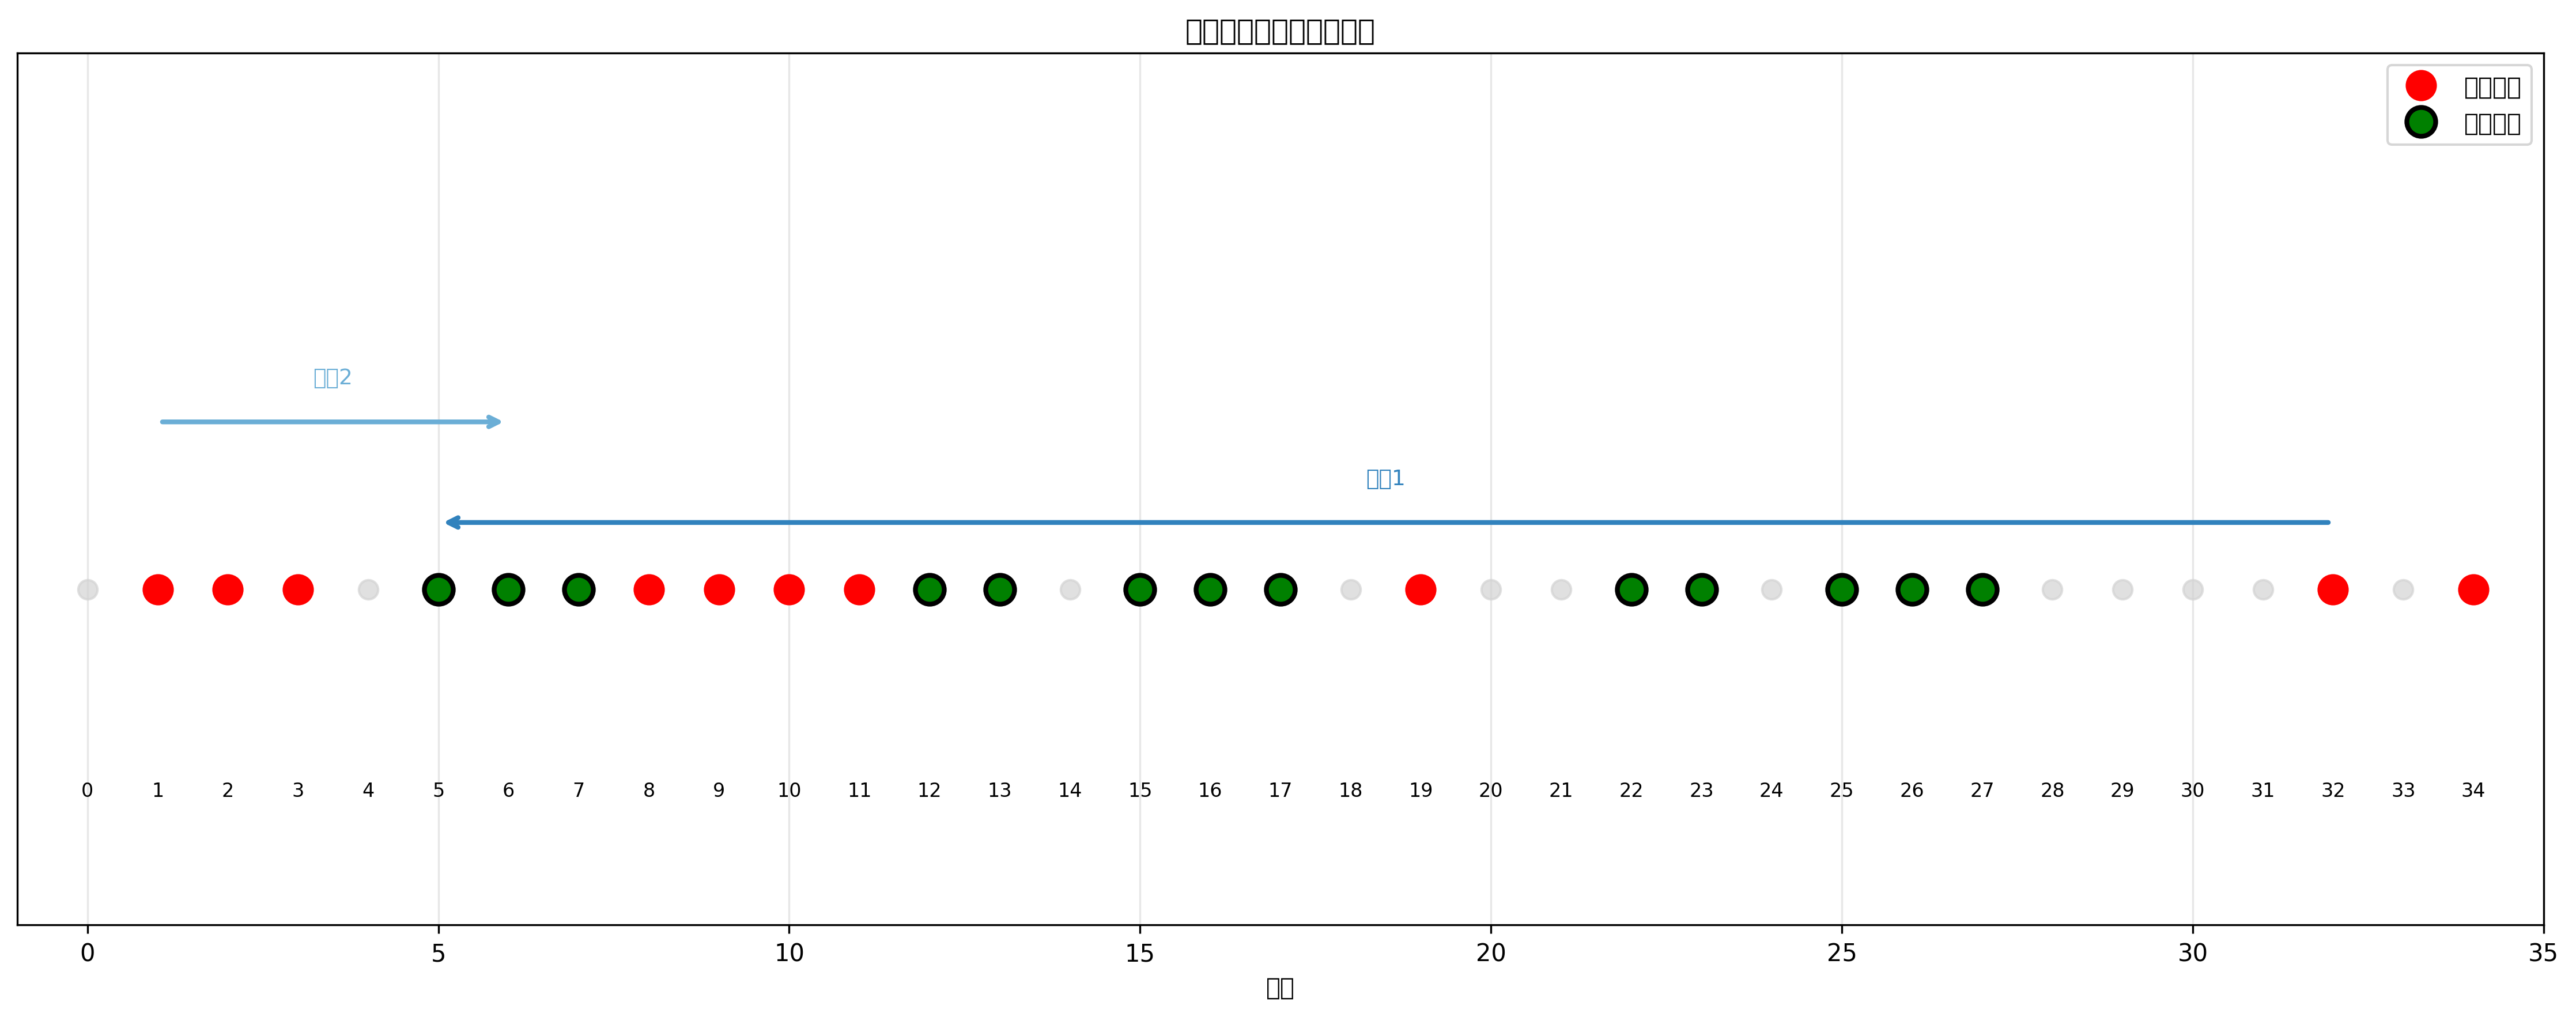
\includegraphics[width=0.92\textwidth]{assets/atom_movement.png}
  \caption{原始 \filepath{PythonCamDemo} 中保存的 atom movement 结果图。它适合放在 planner 章节，因为它展示的不是单个 device call，而是拍图、判别、路径规划和 AOD move 共同作用后的实验现象。}
\end{figure}


\begin{figure}[htbp]
  \centering
  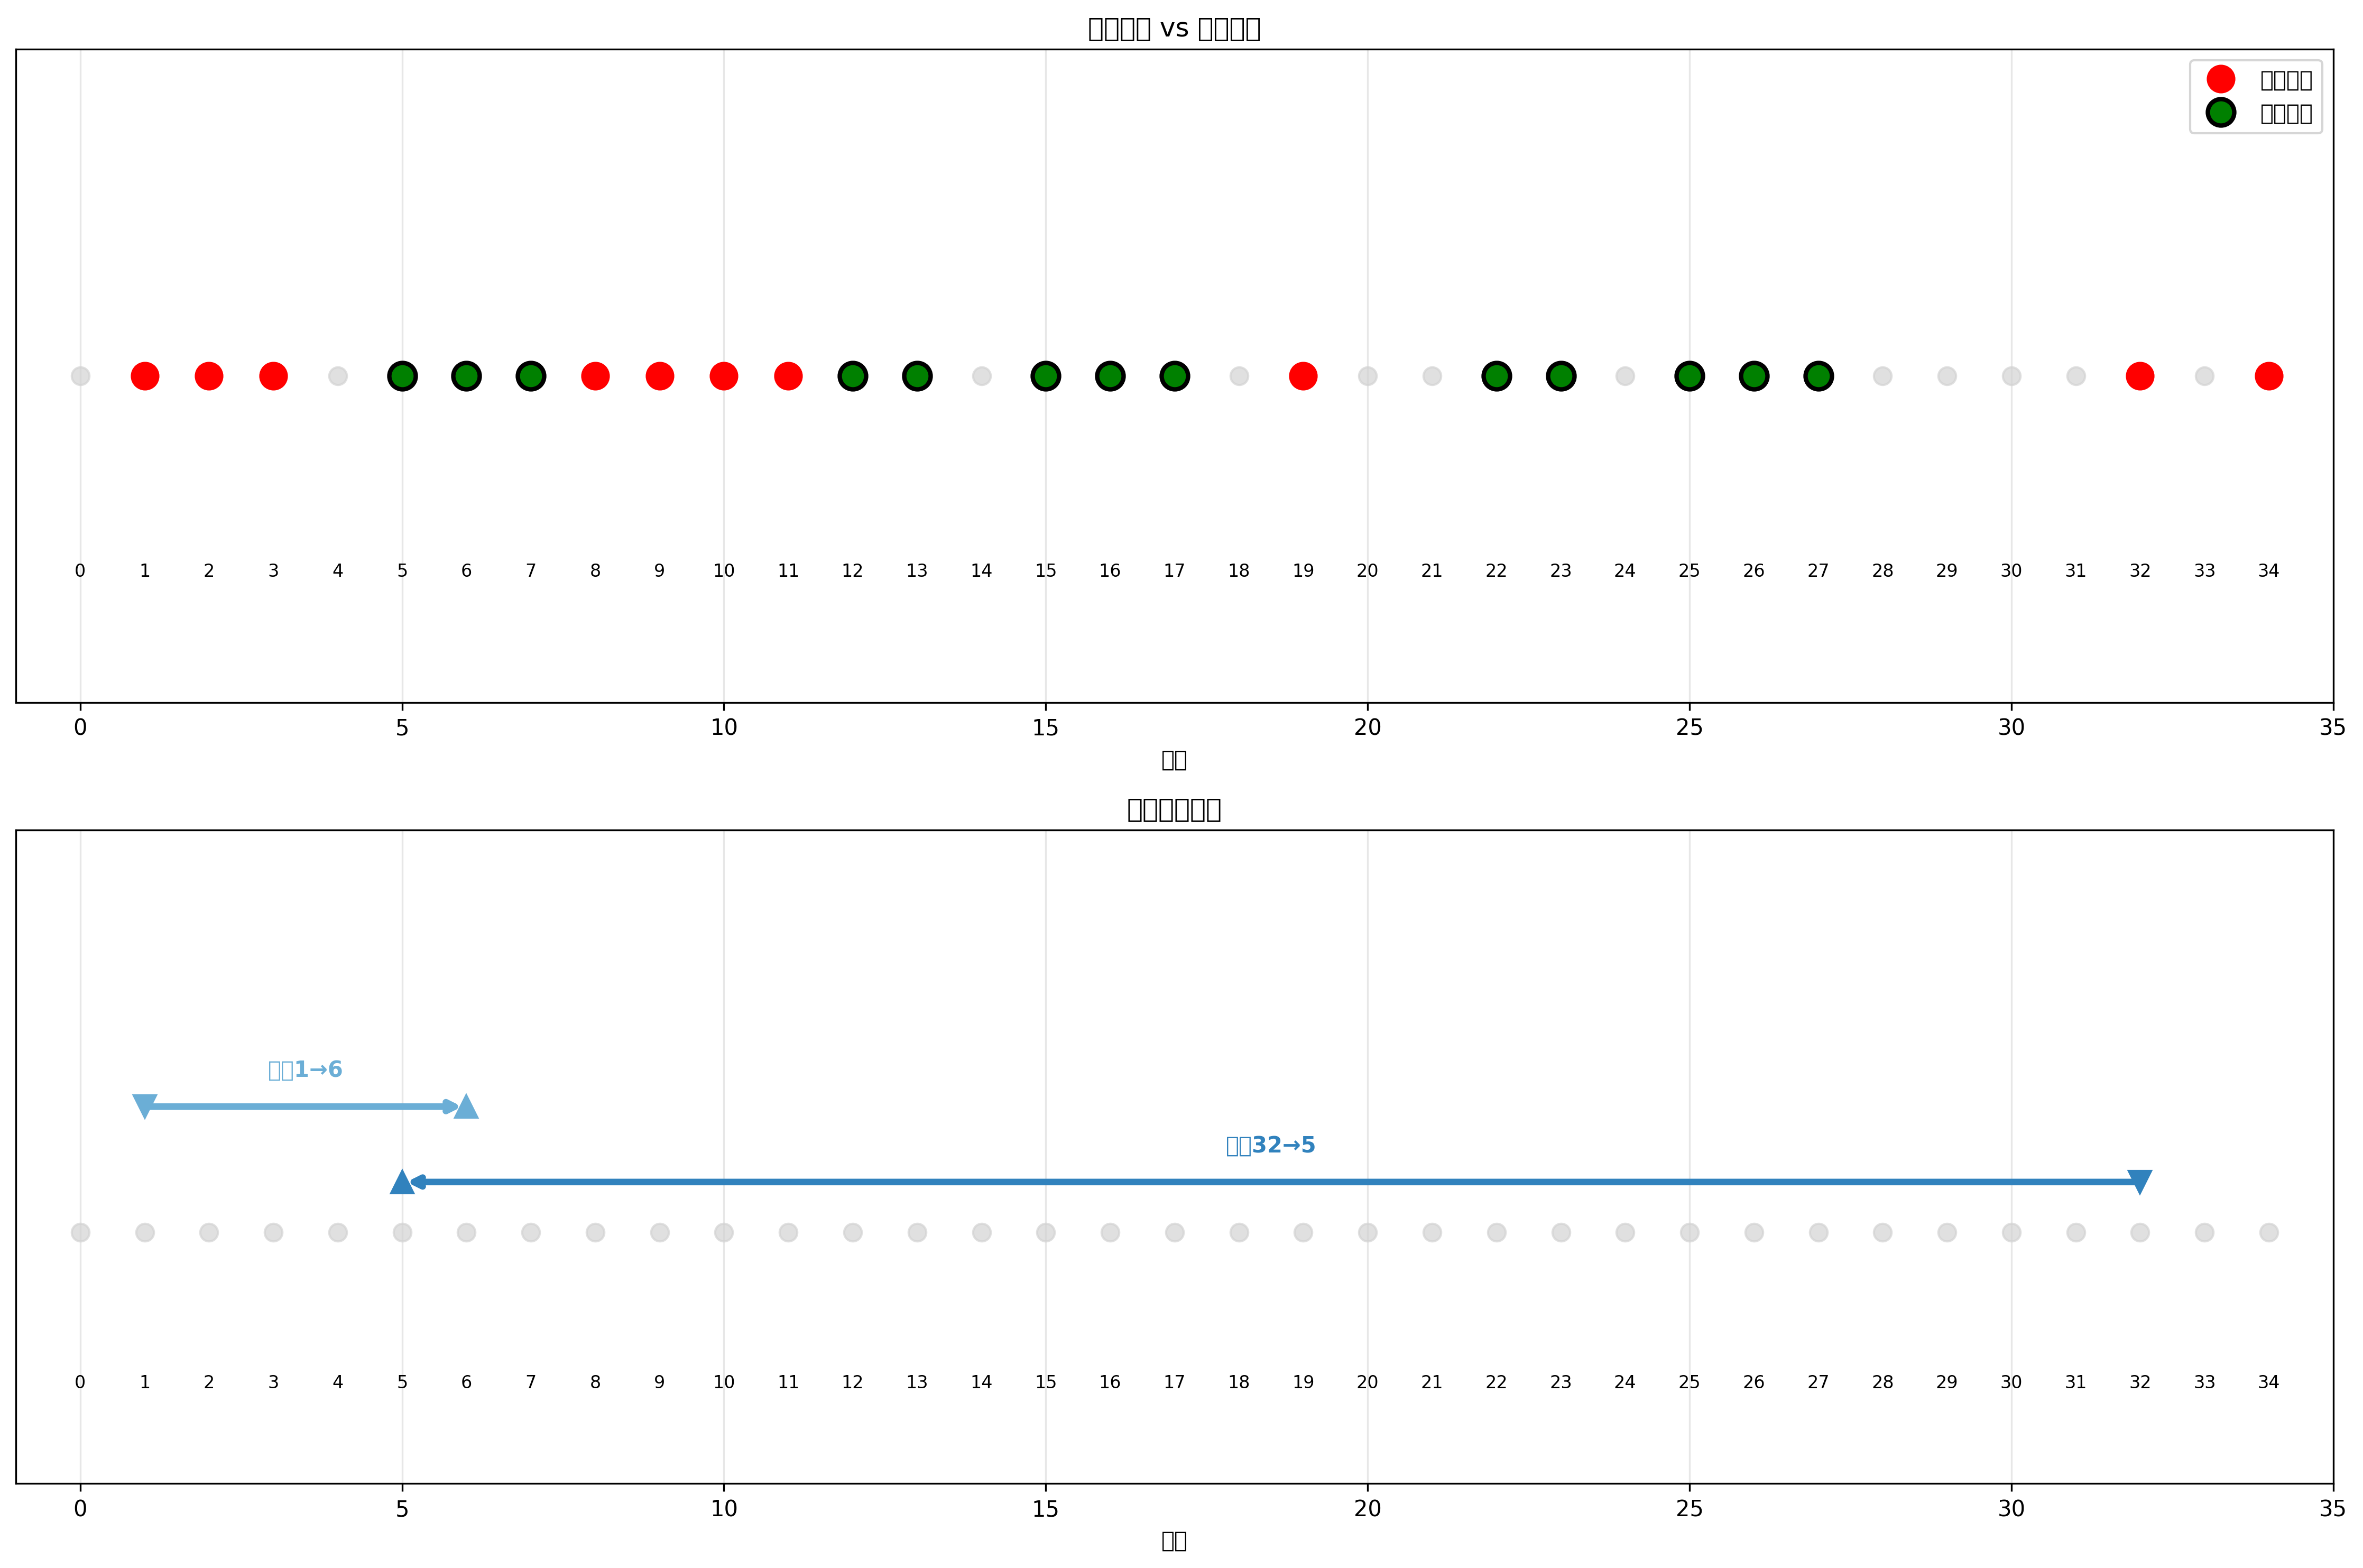
\includegraphics[width=0.92\textwidth]{assets/atom_movement_enhanced.png}
  \caption{原始结果图的增强版。重构后的 run record/plot 接口要保留这种实验可读性，同时把图背后的 pulse、threshold、frequency map 和 move trace 一起保存。}
\end{figure}


\section{planner 和 hardware move 的边界}
原始代码中 planner 输出和 PXIE move 调用常常在一个 notebook cell 里直接相连：\pyapi{atom_path} 生成后马上调用 \pyapi{move_atom(pxie, atom_path, frequency_AOD)}。这很直观，但也意味着 planner 错误、frequency map 错误和 PXIE DLL 错误会在同一层爆炸。

重构把这三件事分开：
\begin{itemize}
  \item \pyapi{plan_rearrangement} 只在 site-index 空间工作，输出 \pyapi{RearrangementPlan}。
  \item \pyapi{FrequencyMap} 负责 site index 到 \pyapi{(f0,f1)} 的映射，并记录 legacy layout。
  \item \pyapi{plan_move} 把 site path 和 frequency map 转成 \pyapi{AODMove} segment table。
  \item \pyapi{PXIEAOD.execute_move} 只负责验证 segment table、调用 DLL 和等待 ramp 完成。
\end{itemize}
这样出错时可以清楚分层：target 越界是 planner 输入问题；frequency map 缺 site 是校准问题；segment 超过硬件上限是 AODMove 参数问题；DLL 返回错误才是硬件执行问题。

\chapter{PXIE/AOD 原始控制逻辑}
\section{DLL 绑定和板卡初始化}
\filepath{pxie_control.py} 通过 \pyapi{ctypes.cdll.LoadLibrary("C:\\Windows\\SysWOW64\\pxie.dll")} 载入 DLL，并给每个函数设置 \pyapi{argtypes/restype}。这一步很重要：没有 \pyapi{argtypes}，Python 到 C 的参数传递可能默默错位。

\pyapi{pxie_open} 会打开板卡、设置工作模式，然后初始化很多 SSB 参数。原始代码里 card id 默认是 \pyapi{0x1A0000}，两轴 channel 通常是 0 和 1。重构后的 \pyapi{PXIEAOD} 保留 card id、channels、DLL path 这些参数，但会在构造和 config inspection 阶段检查它们是不是整数、两轴是否重复、wait margin 是否合理。

\section{频率 ramp 的物理含义}
\pyapi{move_caculate_frequency} 和 \pyapi{move_caculate} 是原始 AOD move 的核心。给定起点频率和终点频率，它先算频率差 \pyapi{diff_f}，再根据距离长短选择三段或两段 profile：
\begin{itemize}
  \item 距离长：加速、匀速、减速。
  \item 距离短：加速、减速，没有匀速段。
  \item 不移动：给非常短的占位段或等待段。
\end{itemize}
参数 \pyapi{a} 是 ramp acceleration step，\pyapi{time_a} 是加速段 tick 数，\pyapi{eta = 109.2 * 4 / a} 是从频率差到时间的经验换算。两轴移动时，原始代码分别算 f0 和 f1 的自然耗时，再把较短轴补一个加速度为 0 的等待段，使两轴同时完成。这一点非常关键：AOD tweezer 的二维移动必须保持两轴时序同步，否则实际路径不是 planner 以为的路径。

\section{amplitude ramp up/down}
\pyapi{move_atom} 在正式频率移动前后加了 amplitude ramp：
\begin{enumerate}
  \item 起点 site 的 f0/f1 设置到 SSB。
  \item 先 ramp up，把移动 tweezer 打开。
  \item 执行频率 ramp。
  \item 再 ramp down，把移动 tweezer 关掉。
\end{enumerate}
原始代码中 \pyapi{amp_max = 16500}，ramp step 常见为 \pyapi{23}，ramp time 常见为 \pyapi{45500} tick。RA 参数最终写进 \pyapi{speed0/step0/section0} 和 \pyapi{speed1/step1/section1} 这几个长度 250 的 C int array。section 是累计时间，不是每段 duration。执行后用 \pyapi{time.sleep(max(section0[-1], section1[-1]) * 4e-9)} 等待硬件完成。

\section{丢弃原子}
\pyapi{moveoff_atom} 是把不需要的 atom 移出阵列。它根据 site index 判断在阵列左半边还是右半边，然后沿 f0 方向往外多移一个 margin。这个设计的物理意义是：不需要精确放到另一个 site，只要离开 trapping array，就不会影响目标区域。

\section{重构对应关系}
重构后：
\begin{itemize}
  \item \pyapi{AODMoveParams} 保存 \pyapi{accel/accel_time_ticks/ramp_step/ramp_time_ticks/amp_max/tick_seconds}。
  \item \pyapi{plan_move} 复用“长距离三段、短距离两段、两轴补齐、ramp up/down”的逻辑，但输出结构化 \pyapi{AODMove}。
  \item \pyapi{AODMove.validate} 检查 site path、segment 数、tick 正数、amp 范围和 max segments。
  \item \pyapi{PXIEAOD.execute_move} 在打开/调用 DLL 前先验证 move，执行后把 \pyapi{last_move} trace 写入 snapshot。
  \item \pyapi{VirtualAOD} 使用同样的 move 对象更新 virtual trap occupancy，保证 real/virtual 实验逻辑共用。
\end{itemize}

\chapter{address\_switch 原始 Verilog 逻辑}
\section{工程结构}
\filepath{address_switch} 是 Vivado 工程。核心文件是：
\begin{description}
  \item[\filepath{main.v}] 顶层 module，定义 TTL/DA/shutter 输出端口，实例化 \pyapi{vio_0} 和 \pyapi{time_sequence}。
  \item[\filepath{time_sequence.v}] 真正的时序状态机，输入 VIO timing 参数，输出 TTL、shutter 和 DA 值。
  \item[\filepath{addre.xdc}] 物理 pin 约束，包括 \pyapi{clk -> R4}、\pyapi{probe -> N15}、\pyapi{trig -> R17}、\pyapi{trap -> M17} 等。
\end{description}

\begin{figure}[htbp]
  \centering
  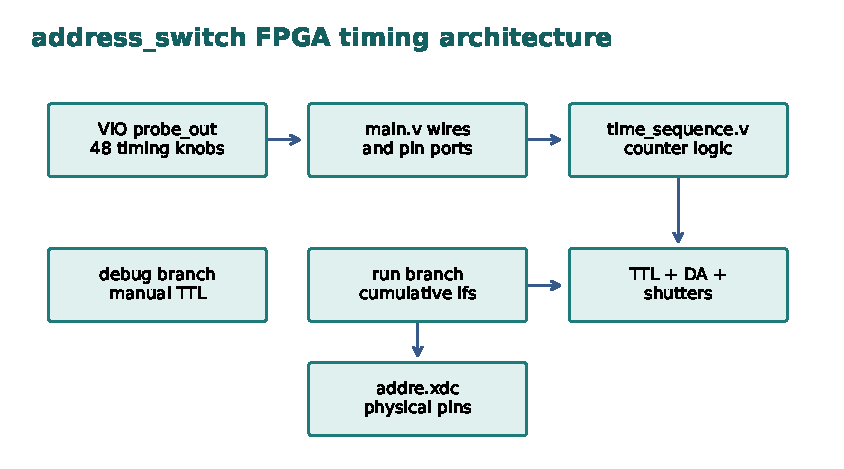
\includegraphics[width=0.96\textwidth]{assets/address_switch_flow.pdf}
  \caption{\filepath{address_switch} 的核心结构：VIO 参数进入 \filepath{main.v}，再驱动 \filepath{time_sequence.v} 中的 counter-based phase logic。}
\end{figure}

\section{main.v: VIO 参数桥}
\filepath{main.v} 的主要工作不是做实验逻辑，而是把 VIO 的 \pyapi{probe_out0..47} 接成有名字的 wire，再把这些 wire 传给 \pyapi{time_sequence}。例如 \pyapi{probe_out2} 是 \pyapi{mot_lasting}，\pyapi{probe_out3} 是 \pyapi{PGC_lasting}，\pyapi{probe_out6} 是 \pyapi{pulse_lasting}，\pyapi{probe_out37/38} 是 Ramsey 参数，\pyapi{probe_out40..42} 是 dipole rampdown 参数。

这个设计的优点是实验员可以通过 Vivado/VIO 动态调 timing 参数，不需要每改一次 MOT 或 PGC 时间就重新综合。缺点是参数名、单位和物理含义只存在于 Verilog wire/comment 里；Python 或 notebook 端无法直接知道当前 VIO 的值，也无法把一次实验的 VIO 参数写入 run record。

\section{time\_sequence.v: 累计时间条件}
\filepath{time_sequence.v} 的 run 分支使用一个 \pyapi{time_count} 计数器。每个实验阶段都写成一个累计时间条件：
\begin{codeblock}[Verilog]
if(time_count == mot_lasting + PGC_waiting) begin
    repump <= 1'b0;
    grey_cooling <= 1'b1;
end

if(time_count == mot_lasting + PGC_waiting + PGC_lasting + probe_waiting) begin
    probe <= 1'b1;
end
\end{codeblock}

这种写法的语义很清楚：MOT、PGC、等待、probe、state prep、microwave、Ramsey、pushout、readout 等阶段沿着一条绝对 tick 时间线发生。但维护风险也明显：如果要在 probe 前插一个阶段，后面所有累计表达式都要检查；如果一个 shutter delay 用负向提前量，表达式中出现 \pyapi{probe_waiting - probe_shutter_open_delay}，需要人工保证不会下溢或跨过其他事件。

\section{debug 分支和 run 分支}
\pyapi{debug} 为真时，\filepath{time_sequence.v} 走手动开关分支：\pyapi{cooling_on/probe_on/address_on/trap_on/...} 等 VIO bool 直接控制 TTL 输出。这适合调线和看单路设备响应。注意 \pyapi{trig} 在现有源码中只在 debug branch 里随 \pyapi{cooling_on} 置高/置低；run branch 中没有显式 \pyapi{trig <= ...} 条件。这意味着真实 qCMOS trigger 在旧工程里要么依赖其他路径/外部接线，要么该端口在 run branch 中不是主控制对象。重构时不能假设旧 \pyapi{trig} 自动就是每帧 qCMOS trigger，而要让 \pyapi{PulseSequence} 中的 \pyapi{trig} 显式出现，并由 preflight 检查 trigger 数量。

\section{TTL、shutter 和 DA 混在同一个时序模块}
旧 Verilog 同时做三类事情：
\begin{itemize}
  \item 数字 TTL：\pyapi{cooling/probe/repump/trap/microwave/pushout/address/emCCD}。
  \item shutter：\pyapi{cooling_shutter/repump_shutter/probe_shutter}，带开关延迟补偿。
  \item analog DA：\pyapi{da_dipole/da_bias_x/y/z}，包括 MOT、trap、pump 磁场值和 dipole rampdown。
\end{itemize}
重构的 Python Verilog 生成器目前只覆盖 TTL timing。DA ramp、磁场值、VIO debug register 这些属于 analog/register control，不应该伪装成 TTL pulse；以后要恢复时，应作为 AOD/analog ramp 或 FPGA register interface 扩展。

\section{pin map 的迁移}
\filepath{addre.xdc} 里的 TTL pin map 是有价值的硬件事实。重构中保留了 address-switch 常量，例如 \pyapi{ADDRESS_SWITCH_PIN_MAP} 和 \pyapi{ADDRESS_SWITCH_CONTROL_PIN_MAP}，并提供 \pyapi{build_address_switch_xdc()}。现在 \pyapi{pin_map} 只描述实验 TTL 输出，\pyapi{control_pin_map} 描述 \pyapi{clk/reset/start/running/done}。这比旧 XDC 中所有端口混在一起更清楚，也能避免把 \pyapi{trigger} 误当成 generated module 的 \pyapi{start}。

\chapter{原始逻辑的关键风险}
\section{不是“代码不好”，而是边界太隐式}
原始代码的问题不是某个实验步骤错，而是很多状态没有明确所有者。下面这张表总结了主要风险和重构中的对应处理。

\begin{tabularx}{\textwidth}{>{\bfseries}p{0.27\textwidth}X}
\toprule
原始风险 & 重构处理 \\
\midrule
qCMOS 打开、采集、显示、保存、平均在同一函数中 & 相机只负责生命周期；图像保存和显示分离；trace 记录每个 stage \\
当前目录决定 \filepath{center.npy/threshold.npy/freq.npy} & \pyapi{TrapCalibration} 和 \pyapi{FrequencyMap} 显式保存路径、layout、metadata 和 hash \\
notebook 全局变量决定当前硬件状态 & \pyapi{DeviceSet} 显式持有 camera/sequencer/aod/trap array \\
没有提前检查 trigger 数和曝光窗口 & \pyapi{preflight_shot} 和 \pyapi{camera.acquire} 双层检查 \\
PXIE path、frequency map 和 DLL 错误混在一起 & planner、frequency map、AODMove、PXIE device 分层 \\
Verilog 手写累计时间表达式容易漏改 & \pyapi{PulseSequence} 先保存物理时间，再统一投影成 edge table \\
实验结果难以复现 & run record 保存 pulse、device snapshot、preflight、calibration hash、Verilog file fingerprint \\
\bottomrule
\end{tabularx}

\section{为什么必须做 preflight}
真实实验中最贵的错误不是 Python 抛异常，而是硬件已经进入一个不确定状态：相机 armed 后没有 trigger、PXIE ramp 还没结束就开始下一步、FPGA 输出了错误 channel、阱频率表和 site ordering 不一致。preflight 的目的不是替代硬件，而是在进入副作用之前尽量确认契约。

重构后的 preflight 检查包括：
\begin{itemize}
  \item device 是否有需要的方法，例如 camera acquire、sequencer prepare/fire、AOD execute\_move。
  \item pulse 是否有重叠、负时间、短于一个 tick 的 pulse 或低电平 gap。
  \item sequence channel 是否被 sequencer channels 覆盖。
  \item qCMOS trigger channel 是否存在，trigger 数是否等于 frames，trigger 间隔是否满足 readout/exposure 预算。
  \item exposure window 是否被 probe/illumination pulse 覆盖。
  \item Verilog channels、pin map、control pin map 和 file name 是否有效。
  \item AOD path 是否有 frequency map，site index 是否越界，segment 是否满足硬件上限。
\end{itemize}

\chapter{重构后的总架构}
\section{模块边界}
重构后的控制层按状态所有权拆分：
\begin{description}
  \item[\filepath{devices.py}] 负责从 JSON/dict/内置模板构造 \pyapi{DeviceSet}。它处理路径、依赖、class registry 和 close 顺序，不做一次 shot。
  \item[\filepath{camera.py}] 负责真实 qCMOS：配置、打开、arm、读帧、stop、trace。
  \item[\filepath{pulse.py}] 负责物理时序：秒、channel、duration、delay、validation。
  \item[\filepath{verilog.py}] 负责 tick-level edge table、Verilog source、XDC、manifest。
  \item[\filepath{sequencer.py}] 负责 \pyapi{prepare/fire} 协议和 generated Verilog bundle。
  \item[\filepath{analysis.py/calibration.py}] 负责 image 到 counts/occupied，以及旧校准文件迁移。
  \item[\filepath{aod.py/rearrangement.py}] 负责 site planner、frequency map、AODMove、PXIE ramp 执行。
  \item[\filepath{experiments.py}] 负责把 device、pulse、analysis 和 frontend 组合成可调用实验。
  \item[\filepath{preflight.py/record.py}] 负责不开硬件的检查和可复查的轻量 run record。
  \item[\filepath{virtual.py}] 负责 virtual camera/sequencer/AOD/trap array，与真实接口保持同名方法。
\end{description}

\begin{figure}[htbp]
  \centering
  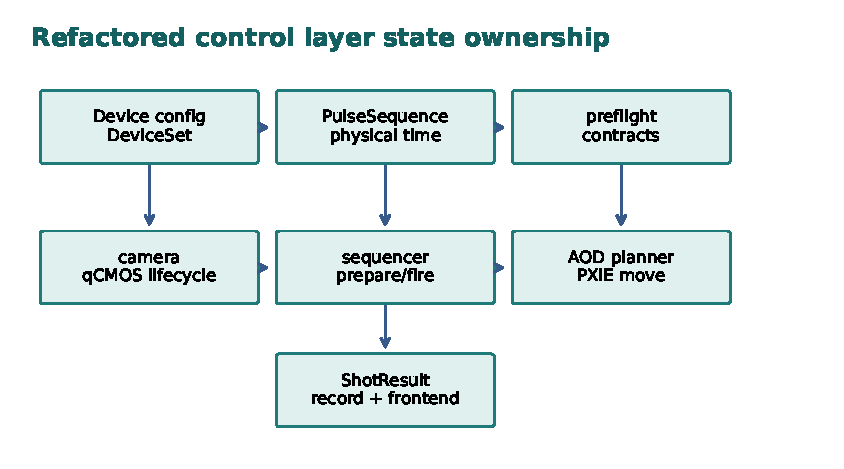
\includegraphics[width=0.96\textwidth]{assets/new_architecture.pdf}
  \caption{重构后的边界：每层只持有自己必须持有的状态，跨层只传小对象。}
\end{figure}

\section{为什么没有一个大 Controller}
中性原子实验很容易诱惑人写一个 \pyapi{MainController}：里面同时保存 camera、FPGA、AOD、calibration、current image、current plot 和 save path。短期看少传参数，长期看会变成所有状态互相引用。真实 bug 会变成“相机 timeout，但也可能是 plot 卡住、PXIE 没等完、threshold 文件错、FPGA trigger 缺失”。

现在的设计刻意保持小对象：
\begin{itemize}
  \item \pyapi{ShotExperiment} 持有 device 和默认 sequence/calibration，但不拥有 Matplotlib artist。
  \item \pyapi{HamamatsuQCMOSCamera} 持有 DCAM handle 和 last trace，但不知道 threshold 怎么判。
  \item \pyapi{VerilogSequencer} 持有 channels、clock、pin map 和 last build，但不知道 qCMOS ROI。
  \item \pyapi{PXIEAOD} 持有 DLL/card/channel 和 last move，但不知道 loading histogram。
  \item \pyapi{DataFigure} 持有 figure/data/fitting，但不知道硬件如何采集。
\end{itemize}
这样每个状态都有明确 owner，debug 时才能沿边界查。

\chapter{实验调度：single shot}
\section{事务流程}
一次 single shot 被设计成一个小事务：
\begin{figure}[htbp]
  \centering
  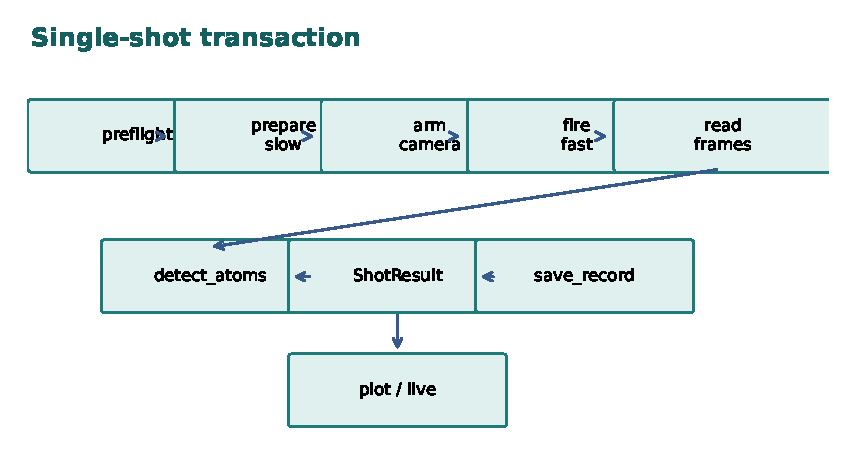
\includegraphics[width=0.96\textwidth]{assets/shot_transaction.pdf}
  \caption{重构后的 single shot 调度：慢动作在 camera arm 前完成，fast fire 在 armed 后执行。}
\end{figure}

\begin{enumerate}
  \item \pyapi{ShotExperiment.acquire()} 选择 sequence、frames、thresholds 和 centers。
  \item 如果 \pyapi{preflight_on_acquire=True}，先跑 \pyapi{preflight_shot}。
  \item \pyapi{camera.acquire(frames, sequence, sequencer)} 进入低层相机边界。
  \item 低层再次检查 sequence 与 sequencer channels、trigger count、exposure window 和 timeout budget。
  \item \pyapi{sequencer.prepare(sequence)} 执行慢动作：生成/写 Verilog、预装载 FPGA、调用 prepare callback。
  \item \pyapi{camera.arm(frames)} 分配 qCMOS buffer 并进入等待触发状态。
  \item \pyapi{sequencer.fire(sequence)} 执行快动作：启动已经准备好的硬件输出。
  \item \pyapi{camera.read_many(frames)} 读取帧。
  \item finally 中 \pyapi{camera.stop()}，保证异常路径也释放 capture 状态。
  \item \pyapi{detect_atoms} 根据 centers/thresholds 得到 counts 和 occupancy。
  \item 返回 \pyapi{ShotResult}，用户再决定 plot/save。
\end{enumerate}

\section{prepare/fire 为什么是核心}
qCMOS 外触发实验里最危险的窗口是 camera 已经 armed 但 trigger 还没来。这个阶段不能再做慢的 Verilog 生成、文件写入、Vivado 下载或 Python 大量计算。因此 sequencer 被拆成两个方法：
\begin{description}
  \item[\pyapi{prepare}] 慢，可以写文件、编译、预装载、检查 callback。
  \item[\pyapi{fire}] 快，只启动已经准备好的 sequence。
\end{description}
如果没有 \pyapi{fire_callback}，真实 \pyapi{VerilogSequencer.fire()} 会报错。这样不会出现“代码看似跑了，但其实只生成了 Verilog 文件，FPGA 没被启动”的假成功。

\section{last\_acquisition trace}
每次 \pyapi{camera.acquire()} 都会留下 \pyapi{camera.snapshot()["last_acquisition"]}。它不是硬件级时间戳，而是 Python 侧事务 trace，包含：
\begin{itemize}
  \item requested frames、sequence name、trigger count/times。
  \item validate/open/prepare/arm/fire/read/stop 阶段的相对时间。
  \item sequencer channel validation 是否执行、错误和 warning。
  \item ROI、exposure、timeout、trigger interval 检查结果。
  \item 实际读到的 frame 数、异常字符串。
\end{itemize}
qCMOS timeout 时先看 trace 停在哪个 stage，而不是直接怀疑 DCAM 或 FPGA。

\chapter{PulseSequence 到 Verilog}
\section{物理时序和 tick 投影分开}
旧 \filepath{time_sequence.v} 直接在 Verilog 里写累计 tick 表达式。重构中先用 \pyapi{PulseSequence} 保存物理语义：channel 名、start 秒、duration 秒、value、channel delay。只有在 \pyapi{validate/compile_edges/generate_sequence_verilog} 时，才把它投影成 FPGA clock tick 和 state mask。

\begin{figure}[htbp]
  \centering
  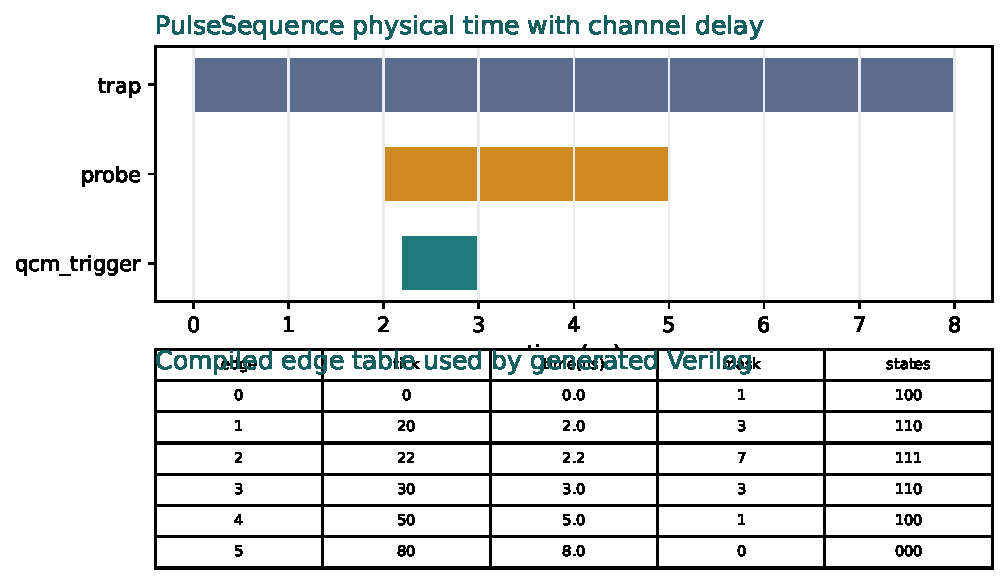
\includegraphics[width=0.96\textwidth]{assets/pulse_projection.pdf}
  \caption{\pyapi{PulseSequence} 先保持秒级物理语义，最后才投影成 edge tick table。}
\end{figure}

这个分离解决几个问题：
\begin{itemize}
  \item 同一个 sequence 可以用于画图、preflight、virtual run、Verilog 生成和 record。
  \item channel delay 只在 \pyapi{effective_events()} 应用一次，避免画图加一次、Verilog 又加一次。
  \item tick rounding 的错误可以集中报告，例如 pulse 短到一个 clock tick 都没有。
  \item record 可以同时保存 raw pulse JSON 和 edge tick 摘要，既能复现物理语义，也能复查硬件投影。
\end{itemize}

\section{VerilogBuild 和 manifest}
\pyapi{generate_sequence_verilog} 会生成 \pyapi{VerilogBuild}，其中包含 module name、channels、clock、ticks、masks、source、source sha256、repeats 和 idle state。\pyapi{write_verilog_bundle} 再写出 \filepath{.v/.xdc/.manifest.json}。manifest 不等于 Vivado project，而是一次生成的轻量 fingerprint：它告诉你这个 Verilog 对应哪些 channel、哪些 edge tick、哪些 pin map、哪些 control ports 和哪份 source hash。

这比旧工程里“Vivado project 当前 VIO 参数是什么”更容易记录。即使真实硬件仍然需要一个外层 wrapper 或下载脚本，Python 侧至少能保证这次 notebook 生成的 \filepath{.v/.xdc} 文件可追溯。

\section{address\_switch 迁移}
旧 \filepath{address_switch} 的全部功能没有一次性搬完。当前重构明确迁移了：
\begin{itemize}
  \item TTL channel 名和 pin map。
  \item legacy tick 参数到秒的转换入口 \pyapi{AddressSwitchTiming.from_legacy_ticks}。
  \item 由 Python 生成 TTL sequence 和 Verilog/XDC 的能力。
  \item clock、pin map、control pin map、file name 的严格验证。
\end{itemize}
没有伪装迁移的是：DA ramp、磁场 analog 值、VIO debug 寄存器、Vivado GUI 内的动态 VIO 调参。这些以后应该作为明确的 analog/register interface 添加，而不是混进 TTL pulse。

\chapter{qCMOS preflight 和同步检查}
\section{trigger 数}
qCMOS 外触发采集最基本的合同是：请求 \pyapi{frames=N}，sequence 中必须有 N 个相机 trigger。原始代码只在 timeout 后知道 trigger 不够；重构中 \pyapi{validate_qcmos_triggers} 会提前从 pulse table 里找 trigger channel，检查 trigger count、width、first trigger time 和 interval。

\section{exposure window}
有 trigger 不等于有有效图。相机曝光窗口必须被 probe/illumination pulse 覆盖。重构中 \pyapi{validate_qcmos_exposure_windows} 会把每个 trigger 后的曝光窗口与指定 exposure channels 的 illumination interval 对比，给出 \pyapi{exposure_windows}、\pyapi{exposure_illumination} 和 \pyapi{exposure_coverage_gaps}。这比只看到一张暗图更可诊断。

\section{timeout budget}
原始代码用固定 \pyapi{timeout_millisec=5000/10000}。重构中 timeout 仍然是配置，但会根据 sequence 的 trigger 时间、exposure 和 readout 间隔估计等待预算。如果预算超过 timeout，会在 preflight/trace 里明确说明。

\section{ROI}
硬件 ROI 是 DCAM subarray，格式为 \pyapi{(x,width,y,height)}。分析 ROI 是 site center 周围的小窗口。二者不能混淆。重构中 \pyapi{QCMOSConfig.validate_roi()} 检查硬件 ROI 的整数性、step、最小尺寸和 sensor shape；\pyapi{detect_atoms} 检查分析 ROI 是否落在图像内。

\chapter{AOD/PXIE 重构}
\section{FrequencyMap}
\pyapi{FrequencyMap} 接管旧 \filepath{freq.npy} 的语义。它可以从 legacy file 载入，并显式指定 \pyapi{layout="freq_list"}、\pyapi{"freq_list1"} 或 \pyapi{"raw"}。layout 会进入 calibration metadata 和 run record，避免 site index 和 AOD frequency 顺序隐式错位。

\section{AODMove}
\pyapi{AODMove} 是“已经规划好的硬件 ramp”。它包含 site path、起始频率、两轴 segment、duration 和参数。planner 输出 site path；\pyapi{plan_move} 输出 AODMove；PXIE 只执行 AODMove。这样用户可以在调用真实 DLL 前打印/保存/验证 move。

\section{PXIEAOD}
\pyapi{PXIEAOD.execute_move(move)} 复用原始思路：设置 SSB 起点、上传 RA segment、启动两轴、等待 duration。不同的是它会在执行前跑 \pyapi{move.validate()}，执行后保存 \pyapi{last_move} trace。trace 包含 site path、segment 数、duration、等待时间和阶段；run record 可以把它保存下来。

\section{VirtualAOD}
virtual AOD 不只是 mock。它接受同一个 \pyapi{AODMove}，更新 virtual trap occupancy，并复用严格输入规则。这样重排实验可以先在 virtual device 上验证 target、planner、calibration 和 record，再换真实 PXIE。

\chapter{frontend 在新调度中的角色}
\section{array 契约}
frontend 不属于原始控制代码，但它是重构后让 notebook 和未来 GUI 解耦的关键。公开数据契约只有：
\begin{itemize}
  \item \pyapi{data_x: (N, coord_dim)}，一维或二维坐标。
  \item \pyapi{data_y: (N, channel_dim)}，测量值。
  \item 未完成点用 \pyapi{NaN}。
\end{itemize}
已有 array 用 \pyapi{zf.plot}；阻塞式采集 handle 用 \pyapi{zf.run}。静态图和 live 图不是两套接口，区别只是 array 是否正在被 session 填充。

\begin{figure}[htbp]
  \centering
  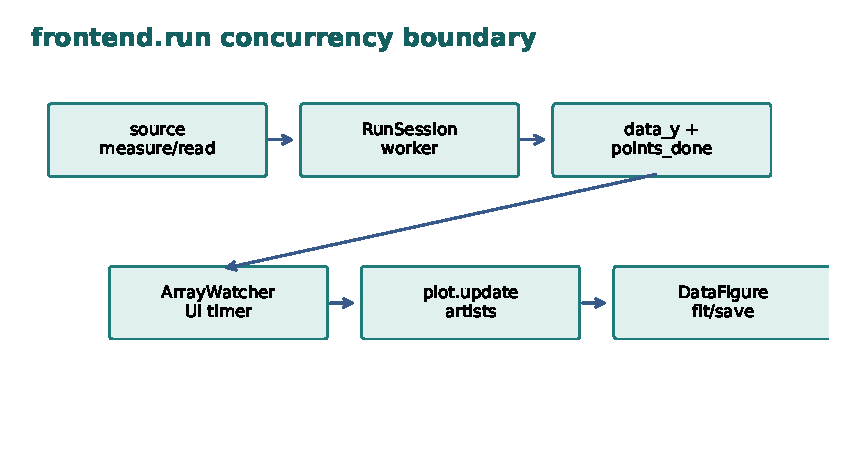
\includegraphics[width=0.96\textwidth]{assets/live_boundary.pdf}
  \caption{重构后的 live 边界：采集 worker 只写 array，UI timer 才更新 Matplotlib artist。}
\end{figure}

\section{为什么不让采集代码自己画图}
Jupyter 中也许可以在采集循环里直接 \pyapi{plot.update()}，但未来 PyQt 中 UI 必须在主线程。重构后的 \pyapi{RunSession} 自己开 worker 调用 \pyapi{measure/read/acquire}，worker 在 lock 下写 \pyapi{data_y} 和 \pyapi{points_done}；\pyapi{ArrayWatcher} 用 Matplotlib/Jupyter timer 在 UI 侧同锁读取 snapshot 并更新 artist。

这解决了用户之前指出的两个核心问题：调用者不需要自己写线程，也不需要把采集函数变成 coroutine；同时图像刷新和硬件 IO 不互相阻塞。2D live 最后缺点的问题也通过 \pyapi{data_y + points_done} 同锁读取解决。

\chapter{run record 和复现}
\section{record 保存什么}
run record 是为了回答“这次实验到底用了什么”，不是为了保存所有 raw data。它保存：
\begin{itemize}
  \item experiment 名、时间、extra metadata。
  \item device snapshot，包括 qCMOS config、sequencer module/pin map、AOD last move。
  \item pulse sequence raw dict、channel delays、validation report、edge ticks。
  \item preflight summary，包括 trigger/exposure/timeout/Verilog checks。
  \item calibration summary，包括 centers/threshold/frequency map 小数组和 hash。
  \item result 摘要，包括 counts、occupied、image shape/min/max。
  \item Verilog/XDC/manifest 文件路径、存在性、大小、sha256 和 manifest 内容。
\end{itemize}
raw camera stack 仍然应该单独保存为 \filepath{.npz} 或 TIFF。record 是索引和 fingerprint。

\section{为什么不保存完整 Verilog source}
完整 source 可能较长，而且磁盘上已经有 \filepath{.v}。record 保存 source hash、file path 和 manifest。这样更适合判断“当前磁盘文件是否还是当时那份”。如果需要完整 source，可以从 manifest 对应路径读取并比对 hash。

\section{snapshot 的意义}
真实设备 snapshot 不是 GUI 状态，而是实验边界状态。例如 \pyapi{VerilogSequencer.snapshot()} 在未 prepare 时也会显示 module name、pin map、control pin map、iostandard、clock 和 output dir；prepare 后显示 prepared sequence 和 repeats。这样 config review 阶段就能发现 pin map 错误，而不是等到硬件没响应。

\chapter{从旧 notebook 到新接口的迁移路线}
\section{单次拍图}
旧写法：
\begin{codeblock}[Python]
dcam = qCMOS_init(exposure_time=0.02, roi=CROP_ROI)
img = qCMOS_EXTERNAL_detect(dcam, buf_alloc=1, timeout_millisec=10000)
qCMOS_end(dcam)
\end{codeblock}
新写法：
\begin{codeblock}[Python]
dev = na.load_devices("virtual")  # or remote_template/custom JSON
shot = na.ShotExperiment(dev, calibration=cal)
result = shot.acquire(sequence=seq)
shot.save_record("results/shot_record.json", result)
\end{codeblock}
差别不是少写几行，而是新写法会在 acquire 前后留下 preflight、trace、calibration 和 record。

\section{多帧 stack}
旧写法中 \pyapi{frames_per_group} 的平均逻辑在 qCMOS capture 函数里。新写法中 \pyapi{ImageStackExperiment} 返回 \pyapi{ImageStackResult}，它知道 raw frames、frames\_per\_group、complete groups 和 sub-frame averages。大数组可以 \pyapi{save_npz}，轻量 JSON 仍然走 \pyapi{save_record}。

\section{重排}
旧写法：
\begin{codeblock}[Python]
img_before = qCMOS_EXTERNAL_detect(dcam)
array = find_atom(img_before, center, threshold)
move_step, start_positions = compress_algorithm(array, target, atom_site)
for atom_path in move_step:
    move_atom(pxie, atom_path, frequency_AOD)
img_after = qCMOS_EXTERNAL_detect(dcam)
\end{codeblock}
新写法：
\begin{codeblock}[Python]
rearrange = na.RearrangementExperiment(shot, dev.aod, frequency_map=fmap)
report = rearrange.preflight(targets)
report.raise_if_failed()
result = rearrange.execute(targets)
\end{codeblock}
新写法的重点是 preflight 分两段：拍 before 前检查 targets/AOD/frequency map，拍 before 后根据实际 occupied sites 规划 path 并检查 move。

\section{address\_switch}
旧写法靠 Vivado/VIO 参数。新写法推荐先把一个实验阶段写成 \pyapi{PulseSequence}，再生成 Verilog bundle：
\begin{codeblock}[Python]
seq = na.default_imaging_sequence(exposure=20e-3)
sequencer = na.VerilogSequencer(
    channels=["trap", "probe", "trig"],
    pin_map={"trap": "M17", "probe": "N15", "trig": "R17"},
    control_pin_map={"clk": "R4"},
)
build = sequencer.prepare(seq)
\end{codeblock}
如果要迁移旧 tick 参数，用 \pyapi{AddressSwitchTiming.from_legacy_ticks(clock_hz=...)}，把 tick 数转换到秒，再统一进入 \pyapi{PulseSequence}。

\chapter{调试地图}
\section{按症状查层}
\begin{description}
  \item[import 或配置失败] 看 \pyapi{inspect_device_config}、device class、参数名、path-like 参数和 \pyapi{"$device:name"} 依赖。
  \item[qCMOS timeout] 先看 \pyapi{last_acquisition.stage_timings} 停在哪一步，再看 trigger count、timeout budget、sequencer fire 错误。
  \item[有图但很暗] 看 exposure window 和 illumination channels，不要先怀疑 threshold。
  \item[检测 occupancy 错] 看 calibration centers、ROI radius、reducer、threshold 长度和 center ordering。
  \item[AOD 移错 site] 看 FrequencyMap layout、site path、AODMove segment 和 PXIE \pyapi{last_move}。
  \item[Verilog 图对硬件不对] 看 clock\_hz、edge ticks、pin map、control pin map、manifest hash 和 wrapper/Vivado 连接。
  \item[live 图最后少点] 看 frontend 的 \pyapi{points_done}、lock 和 \pyapi{ArrayWatcher} snapshot，而不是 imshow。
\end{description}

\section{新增功能放哪里}
\begin{itemize}
  \item 新相机属性：放 \pyapi{QCMOSConfig} 和 \pyapi{HamamatsuQCMOSCamera.configure/open/arm}。
  \item 新 TTL 时序：先写 \pyapi{PulseSequence} helper，再扩展 preflight/Verilog 测试。
  \item 新 analog ramp：不要塞进 \pyapi{PulseSequence} TTL；应新增 analog/AOD/register interface。
  \item 新重排 planner：实现新的 planner 函数，仍输出 \pyapi{RearrangementPlan} 或 site paths。
  \item 新图像判别：放 analysis/calibration，返回 counts/occupied，不要写在 camera wrapper。
  \item 新 live 图类型：放 frontend plotter，仍遵守 \pyapi{data_x/data_y} 契约。
\end{itemize}

\chapter{结语}
这次重构不是否定原始 \filepath{PythonCamDemo} 和 \filepath{address_switch}。相反，新的控制层保留了它们最重要的实验事实：qCMOS 外触发、ROI/subframe 平均、center/threshold/frequency map、Hungarian/cascade 重排、PXIE 两轴同步 ramp、address-switch TTL pin map 和硬件时序必须在 FPGA 侧执行。

改变的是软件边界。原始代码把“我现在就要让实验跑起来”做得很好；重构后的代码要让“半年后别人能复现、出错后能定位、换真实/虚拟设备不用重写、接 Jupyter/PyQt 不互相阻塞”也成立。这个目标要求我们把每个状态放在正确的层：相机 buffer 属于 camera，pulse 物理语义属于 PulseSequence，tick 投影属于 VerilogBuild，frequency table 属于 FrequencyMap，site 判别属于 calibration/analysis，显示属于 frontend，实验结果和 fingerprint 属于 record。


\end{document}
